\RequirePackage{tikz}
% Opcje klasy 'iithesis' opisane sa w komentarzach w pliku klasy. Za ich pomoca
% ustawia sie przede wszystkim jezyk i rodzaj (lic/inz/mgr) pracy, oraz czy na
% drugiej stronie pracy ma byc skladany wzor oswiadczenia o autorskim wykonaniu.
\documentclass[english,shortabstract,mgr]{iithesis}

\usepackage[utf8]{inputenc}
\usepackage{ulem}
\usepackage{amsthm}
\usepackage{subcaption}
\usepackage{cite}
\usepackage{float}

\usetikzlibrary{shapes.multipart}
\usetikzlibrary{decorations.text}
\usetikzlibrary{automata}


%%%%% DANE DO STRONY TYTUŁOWEJ
% Niezaleznie od jezyka pracy wybranego w opcjach klasy, tytul i streszczenie
% pracy nalezy podac zarowno w jezyku polskim, jak i angielskim.
% Pamietaj o madrym (zgodnym z logicznym rozbiorem zdania oraz estetyka) recznym
% zlamaniu wierszy w temacie pracy, zwlaszcza tego w jezyku pracy. Uzyj do tego
% polecenia \fmlinebreak.
\polishtitle    {Tłumaczenie współczesnego języka programowania\fmlinebreak do Maszyny Minsky'ego.}
\englishtitle   {Modern programming language translation to the theoretical model of Minsky Machine (Counter Machine).}
\polishabstract {
Maszyna Mińskiego (definiowana jako skończony zbiór stanów i~przejść mięszy nimi, korzystająca
z~dwóch liczników jako pamięcie oraz osobnych liczników odpowiadających za wejście/wyjście) ma
taką samą siłę wyrazu co współczesne języki programowania. To jest znany już fakt, bardziej
popularny w~wersji z Maszyną Turinga. Oznacza to, że dowolny współczesny program da się
przetłumaczyć na teoretyczny model Maszyny Mińskiego (to samo dotyczy Maszyny Turinga).

Moim celem jest zatem zbudowanie automatycznego narzędzia tłumaczącego współczesny język
programowania (Brainfuck) do Maszyny Mińskiego.
}
\englishabstract{
Counter Machine (a machine with finite state set, two counters and input/output counters) is~able
to express any computations done by~modern programming languages. This is the~well-known theorem,
just like computations performed using Turing Machine and means that anything written in a~modern
programming language is possible to~translate into the~theoretical model of Counter Machine
(as well as into Turing Machine).

My goal is to build automatic translation from a~modern programming language (Brainfuck)
to a~Counter Machine.
}
% w pracach wielu autorow nazwiska mozna oddzielic poleceniem \and
\author         {Jadwiga Pokorska}
% w przypadku kilku promotorow, lub koniecznosci podania ich afiliacji, linie
% w ponizszym poleceniu mozna zlamac poleceniem \fmlinebreak
\advisor        {dr Jakub Michaliszyn}
%\date          {}                     % Data zlozenia pracy
% Dane do oswiadczenia o autorskim wykonaniu
\transcriptnum {247906}                     % Numer indeksu
\advisorgen    {dr Jakuba Michaliszyna} % Nazwisko promotora w dopelniaczu
%%%%%

%%%%% WLASNE DODATKOWE PAKIETY
%
%\usepackage{graphicx,listings,amsmath,amssymb,amsthm,amsfonts,tikz}
%
%%%%% WŁASNE DEFINICJE I POLECENIA
%
%\theoremstyle{definition} \newtheorem{definition}{Definition}[chapter]
%\theoremstyle{remark} \newtheorem{remark}[definition]{Observation}
%\theoremstyle{plain} \newtheorem{theorem}[definition]{Theorem}
%\theoremstyle{plain} \newtheorem{lemma}[definition]{Lemma}
%\renewcommand \qedsymbol {\ensuremath{\square}}
% ...
%%%%%

%\usepackage{todonotes}

\newcommand{\todo}[1]{\textbf{TODO:} #1}
\newtheorem*{hypothesis}{Hypothesis}

\begin{document}

%%%%% POCZĄTEK ZASADNICZEGO TEKSTU PRACY

\chapter{Introduction}

\section{Turing Machine}

Modern computers and their abilities nowadays are complex and depend on many different factors
to~perform given computations, like processor technology, software optimizations within given
processor model, input/output communication protocols and many others. This is why if we want
to~state or proof anything about the behaviour of computer programs then we need to~find a~common
language and~general theoretical model representing any type of "computer".

The model is known since 1936 \cite{turing1937computable} when Alan Turing proposed something
called \textbf{Turing Machine}
to represent a~machine that is able to~execute any computations expressible in~terms of~computer program.
It has all positive and~negative properties which belong to~modern programs, i.e. it~is possible
to create a~program which will never stop or~consume infinite amount of memory. The model does not allow
to~solve all the problems -- it~has got the~same limitations in~sense of~creating algorithms
like a~regular computer.

Turing Machine is~a~finite description of~an~algorithm. To perform calculations it uses
a~potentially infinite tape as~its memory -- we have some amount of~tape at~the beginning,
but~we may extend this tape (glue additional tape cells) to~the right end if necessary.
All cells are either blank or~contain a~single letter -- when a~machine starts its
work it has access to $3$ different tapes: \textit{input tape}, \textit{output tape} and
its own tape for calculations.
\textit{Input tape} is readonly and it gives symbols one by one until the~end of an~input word
(we can not move left or right explicitly). Similarly \textit{output tape} is writeonly and
when a~machine finishes its work there is output word written (if any is needed). Using its regular
tape for computations a~machine can do anything: write, read, move and extend the~tape.
After a~machine finishes (if it finishes at all) it can either \textit{accept}
or~\textit{reject} original input word and there may be an~output word written on output tape
(for simplicity it is usually assumed that there is no output word).

As~an~example we can try to construct a~Turing Machine recognizing all binary palindromes of~even length,
formally defined as a~set $A = \{ ww^R : w \in \{0,1\}^* \}$ (where $^R$ means reversing given word).

Because we need to use finite description we say that the~machine should read whole input word
from the~input tape, store it on its computations tape and move to the~beginning of its tape.
Then the~machine should check the~first letter $a_1$ with the~last one $a_n$ -- if these cells
contain different letters then the~machine should immediately reject the whole word,
otherwise it should mark both $a_1$ and $a_n$ as checked (i.e. write $\#$ symbol in~their cells)
and~continue with $a_2$ and~$a_{n-1}$. At~the~end we should have a~tape full of $\#$s and~the~machine
should accept given word. If there is just one unchanged cell left then it was a~palindrome
of~odd length and~we should reject it.

For simplicity we assume we do not have the~output tape -- a~machine may either accept or reject
an~input word written on the~input tape. \textbf{Turing Machine} is a~$6$-tuple
$(Q,\Sigma,\Gamma,\delta,q_0,P)$ where:
\begin{itemize}
  \item $Q$ is~a~finite set of~states the~machine can be within,
  \item $\Sigma$ is~a~finite input alphabet (does not contain blank),
  \item $\Gamma$ is~a~finite tape alphabet and~$\Sigma \subset \Gamma$,
  \item $\delta: Q \times \Gamma \times \left( \Sigma \cup \{\perp\} \right)
      \rightarrow Q \times \Gamma \times \{L,R\} \times \{-,R\}$  is~a~finite
      transition function, $L$ and~$R$ mean the~machine should move one cell
      left or~right respectively,
  \item $q_0$ is~the~initial state the~machine starts within,
  \item $P$ is~a~finite set of~states which accept the~input word.
\end{itemize}

\textbf{Configuration} of~a~Turing Machine consists of ($w$, $q$, $k$), where:
\begin{itemize}
  \item $w \in \Gamma^*$ is a~word written on~the~computations tape,
  \item $q$ is a~state of the~machine is~currently within,
  \item $k$ is a~cell number the~machine is currently looking at.
\end{itemize}

Having a~configuration we can precisely say what is the~program execution progress.
One configuration is~a~precise step of~computation, so a~sequence of~configurations (where
each consecutive pair obeys $\delta$) is called
a~\textbf{run} of~a~Turing Machine. This sequence may be finite or~infinite the~same way like
a~program may loop forever or~finish within some number of~steps. Each such run begins with
a~configuration where some word $w$ is~an~input, $k = 0$ which is the~leftmost cell on~the~tape
and~$q = q_0$ which is initial state defined in~the~description of~given machine. If~a~run is
finite and~ends with configuration ($w_n$, $q_n$, $k_n$) then we define the~input word to~be
\textit{accepted} if $q_n \in P$ ($q_n$ is one of accepting states) and \textit{rejected} otherwise.

\section{Church-Turing thesis and Turing-completeness}

Computers are used to perform calculations for us. we want them to~execute some
procedures or~to~perform some process and~we call it an~\textit{algorithm} in~its intuitive meaning.
A~good example could be~a~mathematical problem of~generating prime numbers -- it~is fairly simple
to~think of~a~method of~generating prime numbers by checking lager and~larger numbers and~checking
their all possible divisors. We~are able to~precisely say what this algorithm looks like and~if
we think for a~while we would probably be able to~express it in terms of Turing Machines. That
is~exactly what \textbf{Church-Turing thesis} (see Chapter Church-Turing Thesis of \cite{sipser2012ChurchTuring}) states:

\begin{hypothesis}
  Intuitive definition of~any~algorithm a~human/computer can follow is~equivalent
  to~some description of~Turing Machine.
\end{hypothesis}

This thesis allows us to~think about defining algorithms in~intuitive way while still staying
within the~world of~Turing Machine programs.

It~turns out that when designing any~modern algorithms we use~the same way of~intuitive description
of~a~procedure and~then we~are converting it~into \textit{implementation} which is~a~representation
of~given algorithm using a~modern programming language. From thesis above we~claim that most probably
it~would be~possible to~express it~as~a~Turing Machine (but probably require lots of~thought).

To~avoid~a~painful process of~expressing algorithms in~an~unhandy theoretical model we~have
a~concept of~\textbf{Turing-completeness}. All popular modern programming languages are proven
to~be Turing-complete which means that we are able to~implement our algorithm in~such
language if and only if there exists some equivalent Turing Machine description.

\section{Counter Machine}

We have so far theoretical model -- Turing Machine -- which has the~same power of~expression
as~modern languages and~it turns out there are many others we~can describe and~prove they are
equivalent to Turing Machine (so~to~modern languages as~well). One of~such alternatives
is~\textbf{Counter Machine} (sometimes called \textbf{Minsky Machine}) \cite{minsky_67}
which is~really basic in~its construction.

Similarly to~Turing Machine, Counter Machine has~finite description -- finite set of~states $Q$
and~transition function $\delta$ defining when the~machine may move from one state to~another.
Instead of~the~infinite tape there are $2$ counters -- each counter works like a~glass of~coins,
the~machine may throw a~coin (or~several coins) into the~glass, check whether the~glass is~empty
or~take out a~coin (only one and~only if glass is not empty). Each counter is~basically a~non-negative
integer, but the~machine is~not allowed to~explicitly check its value, it~just gets a~boolean
information about whether it equals $0$.

There are a~few alternative models -- if~we~allow the~machine to~use $3$ counters instead of~$2$
then we get equivalent model, the~same for $4$ or~more counters. According to~this fact, we~can
choose how many counters it~is convenient for~us to~use. The~only exception is~Counter Machine with
$1$ counter which is~not able to~express everything a~$2$ Counter Machine can. As~an~argument
we may say that halting problem for $1$ Counter Machine is~decidable -- it is possible to~check
in~polynomial time whether given description of $1$ Counter Machine will loop forever or~not.
Of~course halting problem for $2$ Counter Machine (which is~equivalent to~Turing Machine model)
is proven to~be not decidable. \cite{minsky_67}

\section {2 stack pushdown automaton (2 stack PDA)}

Similarly to~Counter Machine, finite description of a~2~stack pushdown automaton (see Chapter Context-Free Languages, Pushdown Automata of \cite{sipser2012ChurchTuring})
contains number of~states and~transition function $\delta$, but~counters are replaced with 2 stacks.
These 2~stacks use stack alphabet $\Gamma$ and the~automaton may change their state
by~pushing zero or~more symbols at the~top or~removing \textbf{exactly one} symbol from
the~top.

In practice the~implementation assumes that a~single transition \textbf{always} takes
a~symbol from each stack and after transitioning to a~new state pushes some symbols
(maybe the~original ones) to each stack.

Each stack has a~special symbol $\perp$ at the~bottom that determines when a~stack becomes
empty. Additionally it is not allowed to take $\perp$ out from the stack, so~after transitioning
to a~new state $\perp$ must be pushed back (maybe followed by other symbols) to~the~stack.

Formally 2 stack PDA is a~$6$-tuple ($Q$, $\Sigma$, $\Gamma$, $\delta$, $q_0$, $F$) where:
\begin{itemize}
  \item $Q$ is a~finite set of states,
  \item $\Sigma$ is a~finite input alphabet ($\epsilon \in \Sigma$),
  \item $\Gamma$ is a~finite stack alphabet ($\perp \in \Gamma$),
  \item $\delta: Q \times \Sigma \times \Gamma \times \Gamma \rightarrow
      Q \times \Gamma^* \times \Gamma^*$ is~a~finite transition function,
  \item $q_0$ is the initial state of the~PDA,
  \item $F$ is a~finite set of states which accept the~input word.
\end{itemize}

Each transition specifies when it may be applied by giving a~triple
($a$,~$s$,~$t$)~$\in$~($\Sigma$,~$\Gamma$,~$\Gamma$). It means that input symbol is $a$,
the~left stack has symbol $s$ and the~right stack symbol $t$ at the~top. In practice there
might be multiple transitions matching current state, so it is assumed that the first one
defined is applied.

\section{Brainfuck}

As~we defined above Counter Machine is~a~minimalistic model of~computations, the~same way
\textbf{Brainfuck} \cite{brainfuckWiki} is a~minimalistic (only 8 instructions) programming
language which recalls
the~definition of~Turing Machine -- program operates on~a~tape containing numbers, it~is possible
to~explicitly read and~change values in~cells. A~program operates on~a~data pointer which
points to~the~current focus cell, so~that it~is able to~freely move around. The~main difference
between Turing Machine and~Brainfuck is~lack of~states and~transitions, instead a~program
is a~sequence of intructions that are executed one by~one.

Usually Brainfuck implementations assume that tape length is~around $30\,000$ cells which
is~enough in~most cases. If~we want to~prove Turing-completeness though, this tape
needs to~be potentially infinite. Of couse, no~modern machine is~equipped with infinite memory,
but we are able to~extend it (with buying additional hardware), so~this factor is~omitted
when proving Turing-completeness. It is not a~problem in~this thesis at~all since
the~main goal is to~show that anything written in~modern programming language is~possible
to~automatically translate into~theoretical model.

\section {Purpose of this thesis}

This~thesis should be~a~proof of~theoretical concept based on~Church-Turing thesis -- any~algorithm
or~mathematical method we~are able to~come up with (as~long as it is expressible in any programming
language) is possible to~execute on~the~most basic theoretical model which is a~Counter Machine.

Implementation translates Brainfuck into Counter Machine model and~consists of~a~few separate parts
which are completely separate translations between more and more besic theoretical models.
It is possible to access any transitional (temporary) programs created during the~whole process.

The~plan of translation including transitional models:

\hspace{-1.5cm}
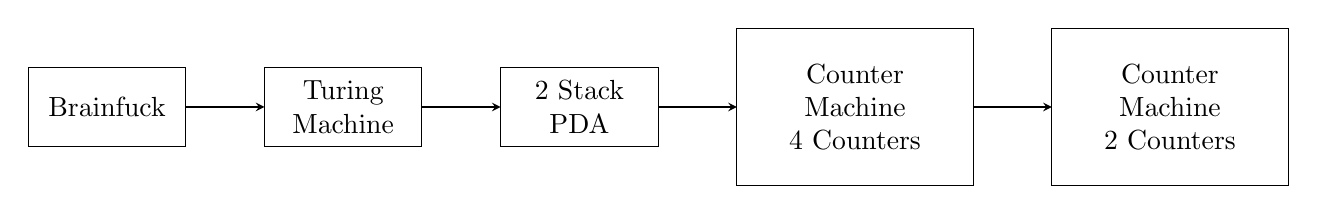
\begin{tikzpicture}
  \draw (0,0) rectangle (2,1) node[pos=.5] {Brainfuck};
  \draw (3,0) rectangle (5,1) node[pos=.5, text width=2cm, align=center] {Turing Machine};
  \draw (6,0) rectangle (8,1) node[pos=.5, text width=2cm, align=center] {2 Stack PDA};
  \draw (9,-0.5) rectangle (12,1.5) node[pos=.5, text width=2.5cm, align=center] {Counter Machine \\ 4 Counters};
  \draw (13,-0.5) rectangle (16,1.5) node[pos=.5, text width=2.5cm, align=center] {Counter Machine \\ 2 Counters};
  \draw [->, >=stealth] (2,0.5) -- (3,0.5);
  \draw [->, >=stealth] (5,0.5) -- (6,0.5);
  \draw [->, >=stealth] (8,0.5) -- (9,0.5);
  \draw [->, >=stealth] (12,0.5) -- (13,0.5);
\end{tikzpicture}

Any two consecutive models have automatic translation, so we may wish to~start with any program written
in Brainfuck, Turing Machine, 2 stack PDA or~4 Counter Machine and receive an~equivalent 2 Counter Machine.
Similarly we may stop at any point of~translations, so it is possible to generate an equvalent program
in 2 stack PDA model from a~program written in Turing Machine model.

The~flexibility in running the~pipeline gives us possibility to prove (as~side-effect)
the~original Church-Turing thesis for Brainfuck. Any~modern program (written in Brainfuck) may be executed
on a~theoretical Turing Machine model.

This paper is organized as follows: Section 2 contains exact specification of all the~models used in translations.
It contains descriptions of how to write source code in each model (i.e. Turing Machine source code). Section 3
explains how we approach each separate translation -- general algorithm to~move from a~source code in one model
to a~source code in the~next one. Section 4 contains technical details about the~implementation -- what tools
were chosen to~this project and how to use the~prepared code. It also discusses encountered problems and presents
a~summary of received results. In section 5 we discuss the~outcome of the~whole work, what could be extended in the~future
and what could be done better with the~current knowledge.

\ldots

\todo{,,Related work''}

\chapter {Preliminaries}

\section {Brainfuck}

Brainfuck is a programming language with only $8$ statements and execution
of~any program is done using a~finite sequence of~memory cells. Statements
operate on~these cells using data pointer --- initially the pointer is set
on the~leftmost cell in the sequence.

Statements:
\begin{itemize}
  \item \texttt{>} moves the data pointer one cell to the right,
  \item \texttt{<} moves the data pointer one cell to the left,
  \item \texttt{+} increase by $1$ the value held in the cell under the data pointer,
  \item \texttt{-} decrease by $1$ the value held in the cell under the data pointer,
  \item \texttt{.} print to stdout the~character that is under the~data pointer,
  \item \texttt{,} read from stdin a~character and write it to the cell under the data pointer,
  \item \texttt{$[$} beginning of a loop with condition checking whether value under
      the~data pointer is zero. If it is then execution jumps to the matching $]$,
  \item \texttt{$]$} closing symbol of a loop --- execution jumps to the~beginning of the~loop
      (matching $[$) and then check for zero value under the data pointer is performed.
\end{itemize}

It is allowed to use any other characters within the code, but anything else than the $8$
listed above are ignored --- it is useful for creating comments in the code.

An example code printing "Hello World!":
\begin{verbatim}
++++++++++
[
>+++++++>++++++++++>+++>+<<<<-
] We set up the values in few cells for future use.
>++.               prints 'H'
>+.                prints 'e'
+++++++.           prints 'l'
.                  prints 'l'
+++.               prints 'o'
>++.               prints space
<<+++++++++++++++. prints 'W'
>.                 prints 'o'
+++.               prints 'r'
------.            prints 'l'
--------.          prints 'd'
>+.                prints '!'
>.                 prints newline character
\end{verbatim}

\section {Turing Machine}

\subsection {Instructions}

Turing Machine consists of a finite number of states, changes between them
and~potentially infinite tape, on~which it is able to~write and~read symbols.
It has no code sequence, a program is a~set of state changes and~definition
of~an~initial state. There is special final state \texttt{END} that does not need
        to~be defined to~be used.

There is a~predefined set of symbols used on the tape which is whole ASCII character set
extended with the same amount of additional (non-ASCII) symbols. Regular
ASCII characters have 7 bits (numbers 0-127), so tape symbols have 8 bits
allowing to hold regular ASCII and special characters (numbers 128-255).

        There are few special definitions (so far using regular ASCII,
but it will be changed to use special characters instead \todo{revisit}):
\begin{itemize}
  \item \texttt{BLANK} which represents empty field on the tape
  \item \texttt{*} (ALL) defines all characters (both ASCII and special)
  \item \texttt{\#} (NOTHING) means no character which is used to say
                   that we do not want to write anything on tape during
                   this state change
          \item \texttt{\&} (NON\_ZERO) defines all characters except 0
          \item \texttt{0} (ZERO) represents zero that is used for conditional jumps
           (jump zero)
          \item \texttt{>} (NEXT\_CHAR) allows writing on the tape next character
                   (increased by one), i.e. writes \texttt{g} if on the tape
                   was \texttt{f}
  \item \texttt{<} (PREV\_CHAR) similarly as above but writes the previous character,
                   i.e. writes \texttt{e} when seen \texttt{f}
\end{itemize}

Defining initial state:
\begin{verbatim}
START: state_name
\end{verbatim}

Each state change looks as follows:
\begin{verbatim}
state_name symbol(s) -> target_state head_move symbol_to_write
\end{verbatim}

\texttt{symbol(s)} is ASCII character including special definitions (currently
all special definitions use regular ASCII so that it is easy to see
in a~standard text file), in future it will allow getting non-ASCII special
characters as well.

\texttt{head move} is one of \texttt{L}, \texttt{R} or \texttt{-} which
steer the head to go left, right or stay in place, respectively.

\texttt{symbol to write} is any (currently ASCII) symbol. Currently, there
is no mechanism to prevent writing any symbol from special definitions,
but~it will cause an~undefined behaviour of~the machine. The only symbol
from special definitions that is allowed to appear as \texttt{symbol\_to\_write}
is \texttt{\#} (NOTHING) meaning that symbol on the tape should not change.

\subsection {Extensions of the theoretical model}

Standard input/output handling is done by allowing to read or write single
ASCII character from/to stdin/stdout. It is possible to~add additional
reading or~writing before moving the~head. It is done by modifying change
symbol \texttt{->} in the~state change definition.
\begin{itemize}
  \item Reading is done with \texttt{->*}, i.e. \texttt{state1 A ->* state2 R NOTHING}
        which means when seen symbol \texttt{A} in state \texttt{state1} we read
        from stdin one character, overwrite \texttt{A} to read value and move
        head one field right.
  \item Writing is done similarly with \texttt{->\^},
        i.e. \texttt{state1 A ->\^\ state2 R NOTHING} which will print symbol
        \texttt{A} on stdout and move the~head to the~right.
\end{itemize}

\subsection{Example}

A~program that reads a~letter from stdin, writes this letter into
stdout and if the~written letter was \texttt{B} or \texttt{b} then prints
\texttt{.} at the end as well, otherwise finishes.

\begin{verbatim}
START: s1
s1 ALL ->* s2 - NOTHING
s2 ALL ->^ s3 - NEXT_CHAR
s3 ALL -> s4 - NOTHING
s4 b ->^ s5 R NOTHING
s4 B ->^ s5 R NOTHING
s5 ALL -> s6 - .
s6 ALL ->^ s7 - NOTHING
s7 ALL -> END - NOTHING
\end{verbatim}

Note: If there is no state change defined for given configuration
(nothing matches) then it is assumed that machine gets to \texttt{END} state.
Because of this in the above example, last instruction is not necessary.

\section {2 Stack Pushdown Automaton}

2 Stack Pushdown Automaton consists of two stacks, input tape and~definition
of~states and transitions between them. Each transition looks as follows:
\begin{verbatim}
state_name left_pattern right_pattern ->
    target_state left_stack_items right_stack_items
\end{verbatim}

Explanation:
\begin{itemize}
  \item \texttt{left\_pattern} is symbol or pattern that should be matched
      for the symbol at the top of the left stack
  \item \texttt{right\_pattern} is the same as above, but for the right stack
  \item \texttt{left\_stack\_items} are the list of items that should be pushed
      to the~left stack before moving to \texttt{target\_state}. It might be
      a~single letter \texttt{"a"}, a~sequence of letters \texttt{"abc"}
      or~sequence of~letters and~references, i.e. \texttt{("a" + ORIG\_LEFT + "b")}
      where \texttt{ORIG\_LEFT} means the letter we read from the~left stack (the one matched
      in \texttt{left\_pattern}). Note: If \texttt{+} is used it is required to put
      the~whole sequence in parenthesis
  \item \texttt{right\_stack\_items} are the same as above, but for items to be pushed into
      the right stack
\end{itemize}

Special references and definitions in transitions:
\begin{itemize}
  \item \texttt{ORIG\_LEFT} is the letter taken from the left stack
  \item \texttt{ORIG\_RIGHT} is the letter taken from the right stack
  \item \texttt{INPUT\_CHAR} is the letter taken from the input tape
      (only in input transition type - see section below)
  \item \texttt{NOTHING} may be used as \texttt{left\_stack\_items} or \texttt{right\_stack\_items}
      and means that nothing is pushed into the left/right stack
  \item \texttt{END} is special state name into which the transition is made if no other transition is specified
  \item \texttt{\$} is the symbol of the stack bottom.
\end{itemize}

\subsection {Extensions of the theoretical model}

Input/Output handling is done similarly to Turing Machine: we change \texttt{->} in transition
to \texttt{->*} or \texttt{->\^}.

When defining input transition it is allowed to use \texttt{INPUT\_CHAR} in any items
to be pushed into left/right stack. Here is an~example that takes a~character from input
tape and pushes it into the~left stack (and ignores symbols taken from both stacks).
\begin{verbatim}
state1 ALL ALL ->* state2 INPUT_CHAR NOTHING
\end{verbatim}

When defining output transition we \textbf{must} specify what character is printed
with adding \texttt{Output: <letter>} at the very back of transition definition.
An~example that prints letter taken from the~left stack (and ignores what was taken from right stack):
\begin{verbatim}
state1 ALL ALL ->^ state2 NOTHING NOTHING Output: ORIG_LEFT
\end{verbatim}
An~example that prints letter "a" (and ignores what was taken from stacks):
\begin{verbatim}
state1 ALL ALL ->^ state2 NOTHING NOTHING Output: "a"
\end{verbatim}

\textbf{Important note:} Order of defining transition matters. If patterns do not match
a~distinct set of letters then the transition that appeared first is applied.

\subsection{Example}

An~example (equivalent to the example from Turing Machine):
\begin{verbatim}
START: init_state
init_state $ $ -> s1 BLANK NOTHING
s1 ALL ALL ->* s2 INPUT_CHAR ORIG_RIGHT
s2 ALL ALL ->^ s3 ORIG_LEFT ORIG_RIGHT Output: ORIG_LEFT
s3 b $ -> s4 (ORIG_LEFT + BLANK) $
s3 b ALL -> s4 (ORIG_LEFT + ORIG_RIGHT) NOTHING
s3 B $ -> s4 (ORIG_LEFT + BLANK) $
s3 B ALL -> s4 (ORIG_LEFT + ORIG_RIGHT) NOTHING
s4 ALL ALL -> s5 "." ORIG_RIGHT
s5 ALL ALL ->^ s6 ORIG_LEFT ORIG_RIGHT Output: ORIG_LEFT
s6 ALL ALL -> END ORIG_LEFT ORIG_RIGHT
\end{verbatim}

\section {Counter Machine (4 counters)}

Counter Machine consists of $4$ counters each holding non-negative integer,
a~finite number of states and~transitions between them. Each transition
looks as follows:

\begin{verbatim}
state_name (pattern pattern pattern pattern) ->
    target_state (number number number number)
\end{verbatim}

Where:
\begin{itemize}
  \item \texttt{state\_name} is the state in which counter machine needs to be
      within for this transition to be applied,
  \item \texttt{pattern} is one of values \texttt{0}, \texttt{1} or \texttt{\_}.
      \texttt{0} means we expect empty counter, \texttt{1} means we expect non-empty
      counter and \texttt{\_} means that this counter state does not matter, so
      this transition should be applied regardless of this counter state.
  \item \texttt{target state} is the state in which machine will be after
      applying the transition,
  \item \texttt{number} is an~integer from the~range \texttt{[-1, MAX\_INT]} specifying
      what should be added to given counter - it is allowed to decrease counter
      by $1$ only, but it is possible to increase it by any number that can be stored
      in regular integer type.
\end{itemize}

\textbf{Note:} If there are many transitions that may be applied in given state
matching all counters \textbf{the first one} is applied. It means that order
of defining transitions matters.

It is required to give an~initial state of the machine with the following statement:
\begin{verbatim}
START: state_name
\end{verbatim}

\subsection {Extensions of the theoretical model}

Input/Output operations fit in the schema of using counters - input and output
are additional counters which transitions may use in a~similar way as counters are used.

Input transition is defined as follows:
\begin{verbatim}
state_name (counters) input pattern ->*
    target_state (numbers) input_operation
\end{verbatim}

Where:
\begin{itemize}
  \item \texttt{input\_pattern} is one of \texttt{0}, \texttt{1} or \texttt{\_}
      (same as counter pattern) and specifies what should be the state
      of input counter for this transition to be applied,
  \item \texttt{input\_operation} specifies what action should be performed
      on input counter and is one of \texttt{LOAD}, \texttt{-1} or \texttt{NOOP}
      meaning respectively loading a~character from stdin into the input counter,
      decrease input counter by \texttt{1} and leaving input counter untouched.
\end{itemize}

This transition reads from stdin into input counter:
\begin{verbatim}
state1 (_ _ _ _) _ ->* state2 (0 0 0 0) LOAD
\end{verbatim}

These transitions read the~value from input counter and store it in first counter:
\begin{verbatim}
state1 (_ _ _ _) 1 ->* state1 (1 0 0 0) -1
state1 (_ _ _ _) 0 ->* state2 (0 0 0 0) NOOP
\end{verbatim}

Note: It is assumed that transition may just decrease the input counter
and is not allowed to increase its value directly.

Output transition is defined as follows:
\begin{verbatim}
state_name (counters) ->^ target_state (numbers) Output: output_operation
\end{verbatim}

Where:
\begin{itemize}
  \item \texttt{output\_operation} specifies what should be performed
      on output counter and may be one of \texttt{FLUSH} or non-negative number,
      meaning respectively pushing counter to stdout and modifying
      the~value stored in the counter by the~given number.
\end{itemize}

These transitions print character stored in first counter:
\begin{verbatim}
state1 (1 _ _ _) ->^ state1 (-1 0 0 0) Output: 1
state1 (0 _ _ _) ->^ state2 (0 0 0 0) Output: FLUSH
\end{verbatim}

Note: It is assumed that transition may just increase the output counter
and is not allowed to decrease its value directly.


\subsection{Example}

Code that reads a~character from stdin doubles its ASCII value and prints the result.
\begin{verbatim}
START: s1
s1 (_ _ _ _) _ ->* s2 (0 0 0 0) LOAD
s2 (_ _ _ _) 1 ->* s2 (1 0 0 0) -1
s2 (_ _ _ _) 0 ->* s3 (0 0 0 0) NOOP
s3 (1 _ _ _) -> s3 (-1 2 0 0)
s3 (0 _ _ _) -> s4 (0 0 0 0)
s4 (_ 1 _ _) ->^ s4 (0 -1 0 0) Output: 1
s4 (_ 0 _ _) ->^ END (0 0 0 0) Output: FLUSH
\end{verbatim}

\section {Counter Machine (2 counters)}

Counter Machine with 2 counters has the same definition as
Counter Machine with 4 counters, but it is allowed to use only
2 counters, so transitions become of the form:

\begin{verbatim}
state_name (pattern pattern) -> target_state (number number)
\end{verbatim}

Input/Output is handled the same way it is handled in Counter Machine with 4 counters.


\chapter{Theoretical underpinnings}

\section {Reduction from Brainfuck to Turing Machine}

Brainfuck is very similar to Turing Machine, so it is relatively easy to build
a~translation. They both have a~tape and both can read and update symbols in any
cell of the~tape. There are two main differences: representation of states and
input/output handling.

\textit{States representation.}
Brainfuck has a~sequence of instructions that need to~be
executed one by~one in the~given order, while Turing Machine has unordered set
of states and transition function (defining how to move between them). Solution
is to give a~unique name to each instruction and specify transitions between
consecutive instructions. The only exception is a~loop, where depending on
symbol stored in current cell we perform transition to $1$ out of $2$ different states.
This is exactly what Turing Machine model provides -- depending on the~symbol
within current cell we apply appropriate transition.

\textit{Input/Output handling.}
Turing Machine can either accept or~reject given input, so it is necessary to
extend this theoretical model to allow side-effects like reading standard
input and writing to standard output. Even though there is a~way to give
input word (it should be initially written on the tape), this thesis assumes
there is separate source and separate destination for I/O operations.
It means that at any point we may load a~symbol into current cell or~send
any symbol (not necessary the one from current cell) to the~screen. This
way Brainfuck itself handles I/O as well which makes translation straightforward.

\section {Reduction from Turing Machine to 2 stack PDA}

Turing Machine operates on a~tape, while 2 stack PDA operates on 2 stacks, so we need
to come up with some idea how to represent a~tape using 2 stacks. This idea is well-known:
we cut the~tape into two pieces in a~way that current cell is at the~top of the~left stack and all
the cells from the~left side are lower in the~left stack and similarly all cells from the~right side
are stored in the~right stack (cell to the right of the~current cell is the top of the~right stack).

The only problem is the~fact that Turing Machine tape is infinite in one direction.
There is an~exact cell that contains the very last non-blank symbol, so we assume the~tape
ends at this symbol to perform our cut. If Turing machine at any point decides to extend
the tape it needs to first move into new cell (make this cell top of the~left stack in our PDA),
so at this point 2 stack PDA model can simply insert additional new element to the left
stack performing this extension.

It is clear what are the equivalent operations to the ones a~Turing Machine performs.
For example equivalent operation to updating current cell is taking one symbol from
the~top of left stack and push new symbol in its place. Moving one cell to the~right
is equivalent to taking one symbol from the~top of the~right stack and pushing it
into the~left stack -- if the~right stack is empty then we just push new blank symbol
to the~left stack.

\section {Reduction from 2 stack PDA to 4 Counter Machine}

Similarly to the~reduction from Turing Machine to 2 stack PDA we need to simulate
one memory model with the~other one. In this case we need to simulate $2$ stacks
with $4$ counters. More precisely, it is enough to show how to simulate $1$ stack
with $2$ counters and then apply the~same idea to both stacks.

Stack alphabet $\Gamma$ is finite and is of size $N = |\Gamma|$. Each symbol from $\Gamma$ may
be assigned a~unique number starting from $1$ up to $N$ ($0$ is problematic -- it will be
explained later). A~stack is a~sequence of numbers $a = a_0 a_1 a_2 \dots a_{k}$ (where $a_0$
is the~top of the~stack and $a_k = \perp = 0$ is the~stack bottom). Such a~sequence we may
represent as a~single number in a~numeral system with base $\bar{N} = N+1$:

$$ a_0 \cdot \bar{N}^0 + a_1 \cdot \bar{N}^1 + \dots + a_{k} \cdot \bar{N}^{k}
    = \sum_{i=0}^{k} a_i \cdot \bar{N}^i $$

Our left counter will hold whole stack as a~single number and our right counter will be used
to perform operations on the~left one. Because of this representation if we had some symbol $a$
with value $0$ then we would not distinguish between an~empty stack and the~one containing
a single $a$ (more precisely $0$ could represent a~stack containing any number of $a$'s
stored on this stack).

We will need a~few stack operations (and their equivalent
mathods on counters):
\begin{itemize}
  \item \textbf{pop} one symbol from the~top,
  \item \textbf{push} one symbol to the~top,
  \item \textbf{check} what is the~symbol at the~top.
\end{itemize}

To \textbf{pop} one symbol from the~stack we just perform an~integer division by $\bar{N}$ on
the~counter. To~perform this division we will decrease counter by $1$ at each step and every
$\bar{N}$-th step will increase the~helper counter by $1$. When the~original counter becomes empty
then in the~helper counter there is the~result of integer division by $\bar{N}$. Now we just
need to copy the~result from helper counter into the~original one. Whole operation is shown in
Figure \ref{fig:pop_operation}.

\begin{figure}[H]
  \begin{subfigure}[b]{0.4\textwidth}
    \centering
    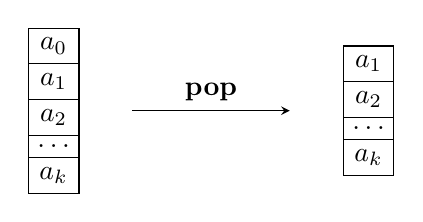
\begin{tikzpicture}[stack/.style={rectangle split, rectangle split parts=#1,draw, anchor=center}]
      \node[stack=5] at (0,0) {
        \nodepart{one}$a_0$
        \nodepart{two}$a_1$
        \nodepart{three}$a_2$
        \nodepart{four}$\dots$
        \nodepart{five}$a_{k}$
      };

      \node[stack=4] at (4,0) {
        \nodepart{one}$a_1$
        \nodepart{two}$a_2$
        \nodepart{three}$\dots$
        \nodepart{four}$a_{k}$
      };

      \draw [->, >=stealth] (1,0) -- (3,0) node [midway, above, sloped] (TextNode) {\textbf{pop}};
    \end{tikzpicture}

    \captionsetup{font=footnotesize}
    \caption{Pop element $a_0$ from the top.}

  \end{subfigure}
  \begin{subfigure}[b]{0.6\textwidth}
    \centering
    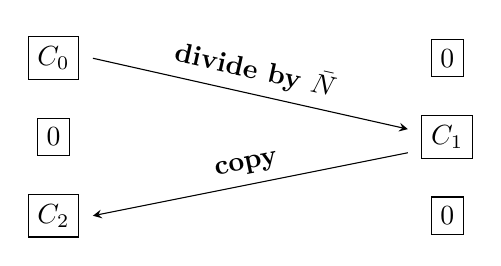
\begin{tikzpicture}[stack/.style={rectangle split, rectangle split parts=#1,draw, anchor=center}]

      \node[stack=1] at (0,2) { \nodepart{one}$C_0$ };
      \node[stack=1] at (5,2) { \nodepart{one}$0$ };

      \node[stack=1] at (0,1) { \nodepart{one}$0$ };
      \node[stack=1] at (5,1) { \nodepart{one}$C_1$ };

      \node[stack=1] at (0,0) { \nodepart{one}$C_2$ };
      \node[stack=1] at (5,0) { \nodepart{one}$0$ };

      \draw [->, >=stealth] (0.5,2) -- (4.5,1.1) node [midway, above, sloped] (TextNode) {\textbf{divide by $\bar{N}$}};
      \draw [->, >=stealth] (4.5,0.8) -- (0.5,0) node [midway, above, sloped] (TextNode) {\textbf{copy}};

    \end{tikzpicture}

    \captionsetup{font=footnotesize}
    \caption{Pop element from the~stack encoded in counter $C_0$.}

  \end{subfigure}

  \caption{Stack vs. counter --- \textbf{pop} operation.}
  \label{fig:pop_operation}

\end{figure}

To \textbf{push} symbol $b$ to the~top of the stack we need to multiply the~counter
by $\bar{N}$ and add number $\bar{b}$ corresponding to symbol $b$:
$$ \bar{b} + \bar{N} \cdot
    \Big[ a_0 \cdot \bar{N}^0 + a_1 \cdot \bar{N}^1 + \dots
    + a_{k} \cdot \bar{N}^{k} \Big]
    = \bar{b} + \sum_{i=0}^{k} a_i \cdot \bar{N}^{i+1} $$
Schematic operations to push stack symbol into a~stack represented as a~number is
shown in Figure \ref{fig:push_operation}.

\begin{figure}[H]
  \begin{subfigure}[b]{0.4\textwidth}
    \centering
    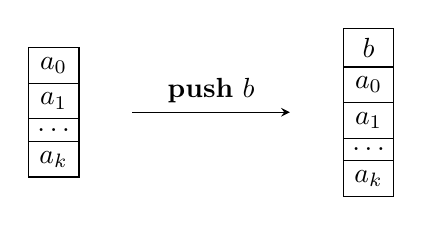
\begin{tikzpicture}[stack/.style={rectangle split, rectangle split parts=#1,draw, anchor=center}]
      \node[stack=4] at (0,0) {
        \nodepart{one}$a_0$
        \nodepart{two}$a_1$
        \nodepart{three}$\dots$
        \nodepart{four}$a_{k}$
      };

      \node[stack=5] at (4,0) {
        \nodepart{one}$b$
        \nodepart{two}$a_0$
        \nodepart{three}$a_1$
        \nodepart{four}$\dots$
        \nodepart{five}$a_{k}$
      };

      \draw [->, >=stealth] (1,0) -- (3,0) node [midway, above, sloped] (TextNode) {\textbf{push} $b$};
    \end{tikzpicture}

    \captionsetup{font=footnotesize}
    \caption{Push element $b$ to the top.}

  \end{subfigure}
  \begin{subfigure}[b]{0.6\textwidth}
    \centering
    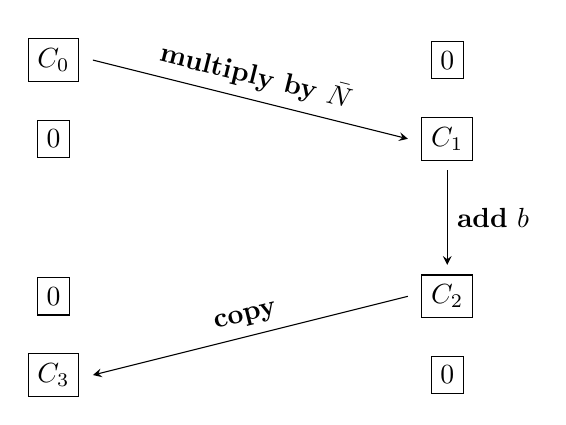
\begin{tikzpicture}[stack/.style={rectangle split, rectangle split parts=#1,draw, anchor=center}]

      \node[stack=1] at (0,4) { \nodepart{one}$C_0$ };
      \node[stack=1] at (5,4) { \nodepart{one}$0$ };

      \node[stack=1] at (0,3) { \nodepart{one}$0$ };
      \node[stack=1] at (5,3) { \nodepart{one}$C_1$ };

      \node[stack=1] at (0,1) { \nodepart{one}$0$ };
      \node[stack=1] at (5,1) { \nodepart{one}$C_2$ };

      \node[stack=1] at (0,0) { \nodepart{one}$C_3$ };
      \node[stack=1] at (5,0) { \nodepart{one}$0$ };

      \draw [->, >=stealth] (0.5,4) -- (4.5,3) node [midway, above, sloped] (TextNode) {\textbf{multiply by $\bar{N}$}};
      \draw [->, >=stealth] (5,2.6) -- (5,1.4) node [midway, right] (TextNode) {\textbf{add} $b$};
      \draw [->, >=stealth] (4.5,1) -- (0.5,0) node [midway, above, sloped] (TextNode) {\textbf{copy}};

    \end{tikzpicture}

    \captionsetup{font=footnotesize}
    \caption{Push element $b$ to the~stack encoded in counter $C_0$.}

  \end{subfigure}

  \caption{Stack vs. counter --- \textbf{push} operation.}
  \label{fig:push_operation}

\end{figure}


The hardest part is to recognize what is the~top symbol -- \textbf{check} operation.
The idea is simple -- we need to calculate the~remainder from division by $\bar{N}$:
$$ \Bigg( \sum_{i=0}^{k} a_i \cdot \bar{N}^i \Bigg) \ \mathrm{mod} \ \bar{N} = a_0 $$
The only place we can remember any information are states. This means that we need
to end up within different state for each remainder -- we call a~state $R_i$ if
recognized symbol has number $i$. Consider example alphabet having $9$ symbols -- Figure
\ref{fig:check} shows all states and transitions needed to~recognize it. Each
transition labelled with $0$ is applied only when counter is empty, similarly
all those labelled with $1$ apply when it is not empty. Additionally when we move around
the~circle (apply transition labelled with $1$) we always decrease the~counter.

\begin{figure}[H]
\centering
\begin{tikzpicture}
\foreach \a in {0,1,...,9}{
  \ifnum\a=0 {
    \node [state,initial] (q0) at (180: 2.5cm) {$q_0$};
  }
  \else{
    \node [state] (q\a) at (-\a*360/10 + 180: 2.5cm) {$q_{\a}$};
  }\fi
}

\foreach \a in {1,2,...,9}{
  \xdef \textplace {right}
  \ifnum\a>4 {\xdef \textplace {left}}\fi
  \ifnum\a=1 {\xdef \textplace {above}}\fi
  \ifnum\a=4 {\xdef \textplace {above}}\fi
  \ifnum\a=5 {\xdef \textplace {above}}\fi
  \ifnum\a=6 {\xdef \textplace {below}}\fi
  \ifnum\a=9 {\xdef \textplace {below}}\fi
  \node [state,accepting] (R\a) at (-\a*360/10 + 180: 5cm) {$R_{\a}$};
  \path[->] (q\a) edge node [\textplace] {0} (R\a);
}

\foreach \a in {0,1,...,9}{
  \xdef \textplace {above}
  \ifnum\a>4 {\xdef \textplace {below}}\fi
  \ifnum\a=0 {\xdef \textplace {left}}\fi
  \ifnum\a=9 {\xdef \textplace {left}}\fi
  \ifnum\a=4 {\xdef \textplace {right}}\fi
  \ifnum\a=5 {\xdef \textplace {right}}\fi
  \path[->] (q\a) edge [bend left=20] node [\textplace] {1} (q\intcalcMod{\a+1}{10});
}
\end{tikzpicture}

\caption{Recognizing symbol from alphabet of size $9$. $R_i$ is the~state with recognized
  symbol $i$, labels on paths define whether counter is empty (0) or not (1).}
\label{fig:check}

\end{figure}

When a~counter value decreases to $0$ then we move to some state $R_i$ (notice that for
correct representations of stacks we never get a~remainder equal $0$, so we never end within $q_0$).
If we do not want to destroy original counter value (which is stack representation) we need
to copy it into our counter for computations and after regognizing symbol at the~top
we need to copy it back to the original counter.

\textit{How to put it all together?}

Because all transitions (in any presented model) are independent, we may focus on a~single
transition and when we build a~translation for it then we can build a~translation for the~whole
program (as long as we keep the~order of transitions).

Each 2 stack PDA transition \texttt{T} has a~\texttt{state} the~model needs to be within,
an~\texttt{other\_state} to which the~model moves into \textbf{if both stack symbol match
the~patterns}.

\begin{verbatim}
state left_symbol right_symbol -> other_state [...]
\end{verbatim}

We will keep state names and build a~new 4 Counter Machine model that will operate as well
on states \texttt{state} and \texttt{other\_state}, but it will have some additional ones
in between. When we want to check whether $T$ should be applied then we perform two
\textbf{check} operations. Because both symbols need to match, after recognizing first symbol
we need to recognize the other without loosing the information about the~first one. This
means that we build a~structure from Figure \ref{fig:check} and in place of each $R_i$ we
paste the same structure for symbols recognition. All unsuccessful paths (symbols not matched)
return to \texttt{state} and successful ones end up within \texttt{other\_state}.

This idea gives O($m^2$) new transitions, where $m$ is the~number of transitions in 2 stack PDA
program. If we consider input counter (which is yet another input stack) then we get O($m^3$)
transitions that we generate. (Fortunately implementation optimizations make it O($m^2$).)

There are still a~few more details to handle:
\begin{itemize}
  \item each applied transition performs a~\textbf{pop} (it always pops a~top element),
  \item transitions may push some items to the stacks (these items may contain symbols that
      were just popped),
  \item a~transition may contain output instruction.
\end{itemize}

Notice that pushing symbols (even few ones) is easy -- we need to apply \textbf{push} operation
multiple times, no matter if it is a~stack or an~output. It is worth to notice
that building this structure takes O($N$) new states assuming the~number of symbols
to push is a~constant. The whole transition $T$ takes O($N \cdot m^2$) newly
generated states.

In practice we want to pop elements together with recognizing them, but now we define the~idea, so
is is enough to say that we perform a~\textbf{pop} after making sure we should apply transition $T$.

\section {Reduction from 4 Counter Machine to 2 Counter Machine}

\todo{Opis}


\chapter{Implementation}

\section{Intruduction}

Language chosen for the entire project is C++, mainly because of its efficiency. Counter Machine
is a~basic model, so any translated program is expected to be very long. These amounts of information
need to be stored and accessed efficiently, so STL library and its containers like hashing table
and hashing set are used havily in this project.

For translation purposes we need to have access to abstract syntax trees of original programs which
means that we should be able to parse a~source code. Most common tools in C++ are Flex and Bison,
for lexing and parsing respectively, which are used in this project. We have several translations
between several different models, so at every step (i.e. Turing Machine to 2 stack PDA) Flex and Bison
are applied to parse a~source code (i.e. in Turing Machine model) and produce abstract syntax tree.
This tree is later used either for evaluation (if we want to execute) or translation to the~next
model in the~pipeline (i.e. 2 stack PDA).

Most of the translations were pretty straightforward and require only basic tricks like
generating unique state names. The~most interesting one was 2 stack PDA to 4 Counter Machine,
which required putting large part of a~program logic into apropriate state names, so it is important
to notice the~structure of the~logic to come up with reasonable translation algorithm.
It turns out that Brainfuck has very specific instructions that allow to make optimizations
to the~translation process.

Few examples:
\begin{itemize}
  \item Input is always a~single symbol and it is directly stored within one of the~memory cells,
      which means we do not need to recognize what is read -- we just blindly store it in memory.
      This is the~optimization mentioned earlier -- we may use only O($m^2$) new states to translate
      a~single 2 stack PDA transition.
  \item From a~given state there might be multiple outgoing paths (a~few different states depending
      on the~stack symbols), but there is no need to build the~whole circle structure for every one.
      We can aggregate all of them and make appropriate outgoing paths to end up within correct
      next states. Notice that for a~single 2 stack PDA transition with explicit symbols (no patterns)
      there is only one outgoing path from our circle structure. In this case instead of wasting all
      the other states $R_i$ we may connect them to appropriate other 2 stack PDA transitions.
      What is more, for all those outgoing paths that do not match any 2 stack PDA transition
      we may just end execution (go to \texttt{END} state).
  \item (partially implemented) If stack is completely ignored by a~transition, there is no point
      to recognize a~symbol on top of it. For example instructions \texttt{>} and \texttt{<}
      in Brainfuck just move to next/previous cell, which in practice ignores the top
      character on one of the~stacks. Another example is an instruction \texttt{+},
      which requires to touch only one of the stacks -- (implemented) for both
      \texttt{+} and \texttt{-} there is only O($m$) new states created.
  \item There is no need to load all the states, becase most probably we will
      not need all of them -- lazy loading allows to add to transition set
      all the transitions that refer to the state that we are currently in.
\end{itemize}

The amount of generated information is very big even for simplest programs, which is not a suprise.
After analyzing for example classical \textit{Hello World!} it turns out that a~human can
significantly reduce the~required logic. Automatic translation will store single letters
in memory (on a~tape or on a~stack) and then print it out, while we may directly use output
tape/stack/counter. This is caused by Brainfuck code structure, where the only thing we can do
is modifying the~memory and then output what is within this memory.

The other problematic operation was shifting Brainfuck's tape --- when we shift
one position our stack in Turing Machine (and later languages) grows by one
character. When we remind ourselves what it means to extend a counter by
one character we realise why is it so -- a counter needs to be multiplyed by
the~size of the~alphabet and increased by the~character's ASCII number.
This means that each time we shift right we increase our counter 140 times
(which is the aplhabet size set within the program) and what is more, next
iterations of a~program need to recognize characters on the top of that
counter with decreasing it by $1$ at a time.

\todo{Wszystko, co było ciekawe}

\section{Technical details}

It is assumed that operating system is Linux -- Debian based distribution. Whole implementation
was tested on Ubuntu and there is no guarantee to work on other platforms.

First requirement is installing Flex and Bison:

\texttt{sudo apt-get install flex bison}

Full handling of each single model is implemented within separate directory called
\texttt{<model>\_parser}, where \texttt{<model>} is short name for the~model
(i.e. \texttt{tm\_parser}). Each directory is a~stanalone part and contains
an~own \texttt{makefile}.

There are $2$ operations allowed for each part:
\begin{itemize}
  \item parse + run -- parse source code and run it: \texttt{./test.e <path\_to\_source\_code>},
  \item parse + translate -- parse source code and translate it into a~source code
      of the~next model: \texttt{./test.e -<next\_model> <path\_to\_source\_code>}.
\end{itemize}

List of commands within directories:
\begin{itemize}
  \item \texttt{bf\_parser}
    \begin{itemize}
      \item run Brainfuck source file: \\ \texttt{./test.e ../examples/hello.bf}
      \item translate Brainfuck to Turing Machine: \\ \texttt{./test.e -turing ../examples/hello.bf}
    \end{itemize}
  \item \texttt{tm\_parser}
    \begin{itemize}
      \item run Turing Machine source file: \\ \texttt{./test.e ../examples/hello.tm}
      \item translate Turing Machine to 2 stack PDA: \\ \texttt{./test.e -2stackPDA ../examples/hello.tm}
    \end{itemize}
  \item \texttt{2stackPDA\_parser}
    \begin{itemize}
      \item run 2 stack PDA source file: \\ \texttt{./test.e ../examples/hello.pda}
      \item (not recommended) translate 2 stack PDA to 4 Counter Machine: \\ \texttt{./test.e -minsky ../examples/hello.pda}
      \item (recommended) translation into multiple files within \texttt{output}
        directory: \\ \texttt{./test.e -multifile output/base ../examples/hello.pda}

        (It will automatically create directory if needed.)
    \end{itemize}
  \item \texttt{mm4\_parser}
    \begin{itemize}
      \item run 4 Counter Machine source file: \\ \texttt{./test.e ../examples/hello.mm4}
      \item (recommended) run source with multiple files (files within \texttt{output}
        directory and created by 2StackPDA translation): \\ \texttt{./test.e -multifile output/base}
    \end{itemize}
\end{itemize}

When we want to run full pipeline then we need to run script \texttt{full\_pipeline.sh} within
\texttt{shared\_files} directory:

\hspace{-1.25cm}
\texttt{./full\_pipeline.sh -f ../examples/hello3.bf -o output/base --run --recompile}

Options:
\begin{itemize}
  \item\textbf{(required)} \texttt{-f <input file path>} or \texttt{--file <input file path>} -- specifies
      the path to input file written in Brainfuck,
  \item \texttt{-o <output file path>} or \texttt{--output <output file path>} -- specifies
      the path to output directory (result of translation) written in 4 Counter Machine. If not
      provided then path \texttt{output/base} is taken -- \texttt{output} directory
      is created and all file names resulted in translation start with \texttt{base}
      and are located within \texttt{output/},
  \item \texttt{-r} or \texttt{--run} -- executes translated code (after translation is completed
      and written to the~specifed output file),
  \item \texttt{--recompile} or \texttt{--clean} forces to recompile all targets,
  \item \texttt{-d} or \texttt{--direct} directly runs translated code written
      in multifile format: \\ \texttt{./full\_pipeline.sh -d output/base}
  \item \texttt{--debug} -- adds additional debugging information when executing program.
\end{itemize}

For details see README.md file included in the~implementation.

\section{Implementation restrictions}

Using multiple files as input is useful to reduce the time and the memory
usage, but it has specific structure that needs to be followed. All the files
within output directory should be created by the provided code, preferably
with \texttt{full\_pipeline.sh} script.

\section{Examples}

\subsection{Brainfuck to Turing Machine}

Classical \texttt{Hello world!} that can be easily found on-line:

\begin{verbatim}
++++++++++
[
>+++++++>++++++++++>+++>+<<<<-
] Na początek ustawiamy kilka przydatnych później wartości
>++.               drukuje 'H'
>+.                drukuje 'e'
+++++++.           drukuje 'l'
.                  drukuje 'l'
+++.               drukuje 'o'
>++.               spacja
<<+++++++++++++++. drukuje 'W'
>.                 drukuje 'o'
+++.               drukuje 'r'
------.            drukuje 'l'
--------.          drukuje 'd'
>+.                drukuje '!'
>.                 nowa linia
\end{verbatim}

It is translated into a~file containing $110$ states (There are long
sequences generated from many consecutive symbols \texttt{+} or \texttt{-} that
were cut for better readability).

\begin{verbatim}
START: state2
state2 ALL -> state1 - NEXT_CHAR
state1 ALL -> state3 - NEXT_CHAR
[...]
state10 ALL -> state11 - NEXT_CHAR
state11 NON_ZERO -> state12 - NOTHING
state11 0 -> state13 - NOTHING
state12 ALL -> state14 R NOTHING
state14 ALL -> state15 - NEXT_CHAR
[...]
state20 ALL -> state21 - NEXT_CHAR
state21 ALL -> state22 R NOTHING
state22 ALL -> state23 - NEXT_CHAR
[...]
state31 ALL -> state32 - NEXT_CHAR
state32 ALL -> state33 R NOTHING
state33 ALL -> state34 - NEXT_CHAR
state34 ALL -> state35 - NEXT_CHAR
state35 ALL -> state36 - NEXT_CHAR
state36 ALL -> state37 R NOTHING
state37 ALL -> state38 - NEXT_CHAR
state38 ALL -> state39 L NOTHING
state39 ALL -> state40 L NOTHING
state40 ALL -> state41 L NOTHING
state41 ALL -> state42 L NOTHING
state42 ALL -> state11 - PREV_CHAR
state13 ALL -> state43 R NOTHING
state43 ALL -> state44 - NEXT_CHAR
state44 ALL -> state45 - NEXT_CHAR
state45 ALL ->^ state46 - NOTHING
state46 ALL -> state47 R NOTHING
state47 ALL -> state48 - NEXT_CHAR
state48 ALL ->^ state49 - NOTHING
state49 ALL -> state50 - NEXT_CHAR
[...]
state55 ALL -> state56 - NEXT_CHAR
state56 ALL ->^ state57 - NOTHING
state57 ALL ->^ state58 - NOTHING
state58 ALL -> state59 - NEXT_CHAR
state59 ALL -> state60 - NEXT_CHAR
state60 ALL -> state61 - NEXT_CHAR
state61 ALL ->^ state62 - NOTHING
state62 ALL -> state63 R NOTHING
state63 ALL -> state64 - NEXT_CHAR
state64 ALL -> state65 - NEXT_CHAR
state65 ALL ->^ state66 - NOTHING
state66 ALL -> state67 L NOTHING
state67 ALL -> state68 L NOTHING
state68 ALL -> state69 - NEXT_CHAR
[...]
state82 ALL -> state83 - NEXT_CHAR
state83 ALL ->^ state84 - NOTHING
state84 ALL -> state85 R NOTHING
state85 ALL ->^ state86 - NOTHING
state86 ALL -> state87 - NEXT_CHAR
state87 ALL -> state88 - NEXT_CHAR
state88 ALL -> state89 - NEXT_CHAR
state89 ALL ->^ state90 - NOTHING
state90 ALL -> state91 - PREV_CHAR
[...]
state95 ALL -> state96 - PREV_CHAR
state96 ALL ->^ state97 - NOTHING
state97 ALL -> state98 - PREV_CHAR
[...]
state104 ALL -> state105 - PREV_CHAR
state105 ALL ->^ state106 - NOTHING
state106 ALL -> state107 R NOTHING
state107 ALL -> state108 - NEXT_CHAR
state108 ALL ->^ state109 - NOTHING
state109 ALL -> state110 R NOTHING
state110 ALL ->^ END - NOTHING
\end{verbatim}

There is clear pattern that each symbol in Brainfuck translates
to a~single transition in Turing machine. The only part which is different
is a~loop:
\begin{verbatim}
state11 NON_ZERO -> state12 - NOTHING
state11 0 -> state13 - NOTHING
state12 ALL -> state14 R NOTHING
state14 ALL -> state15 - NEXT_CHAR
[...]
state42 ALL -> state11 - PREV_CHAR
state13 ALL -> state43 R NOTHING
\end{verbatim}

From \texttt{state11} we have two options (either field on the tape is $0$
or not) and we follow instructions from \texttt{state12} to \texttt{state42}
and then come back to check loop condition once more or we go directly
to \texttt{state13} and skip the body of the loop.

Another example changing uppercase letters to lowercase (by adding $32$
to ASCII number):

\begin{verbatim}
,++++++++++ ++++++++++ ++++++++++ ++.
\end{verbatim}

Automatically translated to:

\begin{verbatim}
START: state2
state2 ALL ->* state1 - NOTHING
state1 ALL -> state3 - NEXT_CHAR
state3 ALL -> state4 - NEXT_CHAR
state4 ALL -> state5 - NEXT_CHAR
[...]
state33 ALL -> state34 - NEXT_CHAR
state34 ALL ->^ END - NOTHING
\end{verbatim}

\subsection{Turing machine to 2 stack PDA}

Further translation of code changing a~character to lowercase:

\begin{verbatim}
START: init_state
init_state $ $ -> state2 BLANK NOTHING
state2 ALL ALL ->* state1 INPUT_CHAR ORIG_RIGHT
state1 ALL ALL -> state3 NEXT(ORIG_LEFT) ORIG_RIGHT
state3 ALL ALL -> state4 NEXT(ORIG_LEFT) ORIG_RIGHT
[...]
state33 ALL ALL -> state34 NEXT(ORIG_LEFT) ORIG_RIGHT
state34 ALL ALL ->^ END ORIG_LEFT ORIG_RIGHT Output: ORIG_LEFT
\end{verbatim}

Note: The order of transitions automatically generated is slightly different,
but because all state names on the~left side of \texttt{->} are distinct
we can do such a~change.

Another example of Turing machine code which rotates letters in english
alphabet by $3$, i.e. for \texttt{a} prints \texttt{d}, for \texttt{A}
prints \texttt{D}, for \texttt{Z} prints \texttt{C} etc.:

\begin{verbatim}
START: init
init ALL -> rotation - NOTHING
rotation ALL -> rotation1 - NEXT_CHAR
rotation1 ALL -> rotation2 - NEXT_CHAR
rotation2 ALL -> rotation3 - NEXT_CHAR
rotation3 ALL -> letters R NOTHING
letters ALL ->* letters1 - NOTHING
letters1 ALL -> change L NOTHING
change 0 -> print R NOTHING
change NON_ZERO -> change1 R PREV_CHAR
change1 z -> change L a
change1 Z -> change L A
change1 ALL -> change L NEXT_CHAR
print ALL ->^ END - NOTHING
\end{verbatim}

Code may be easily changed into a~rotation by any number -- it is enough
to~change \texttt{rotation} sequence to be longer. Suprisingly, this code
is easier to write in Turing machine than in Brainfuck. The~above code
translates to such 2 stack PDA:

\begin{verbatim}
START: init_state
init_state $ $ -> init BLANK NOTHING
change 0 $ -> print (ORIG_LEFT + BLANK) NOTHING
change 0 ALL -> print (ORIG_LEFT + ORIG_RIGHT) NOTHING
change NON_ZERO $ -> change1 (ORIG_LEFT + BLANK) NOTHING
change NON_ZERO ALL -> change1 (PREV(ORIG_LEFT) + ORIG_RIGHT) NOTHING
change1 z ALL -> change NOTHING (ORIG_RIGHT + "a")
change1 Z ALL -> change NOTHING (ORIG_RIGHT + "A")
change1 ALL ALL -> change NOTHING (ORIG_RIGHT + NEXT(ORIG_LEFT))
init ALL ALL -> rotation ORIG_LEFT ORIG_RIGHT
letters ALL ALL ->* letters1 INPUT_CHAR ORIG_RIGHT
letters1 ALL ALL -> change NOTHING (ORIG_RIGHT + ORIG_LEFT)
print ALL ALL ->^ END ORIG_LEFT ORIG_RIGHT Output: ORIG_LEFT
rotation ALL ALL -> rotation1 NEXT(ORIG_LEFT) ORIG_RIGHT
rotation1 ALL ALL -> rotation2 NEXT(ORIG_LEFT) ORIG_RIGHT
rotation2 ALL ALL -> rotation3 NEXT(ORIG_LEFT) ORIG_RIGHT
rotation3 ALL $ -> letters (ORIG_LEFT + BLANK) NOTHING
rotation3 ALL ALL -> letters (ORIG_LEFT + ORIG_RIGHT) NOTHING
\end{verbatim}

\subsection{2 stack PDA to 4 counter machine}

Simple code reading a~symbol and writing it on standard output:

\begin{verbatim}
START: read
read ALL ALL ->* print INPUT_CHAR ORIG_RIGHT
print ALL ALL ->^ END ORIG_LEFT ORIG_RIGHT Output: ORIG_LEFT
\end{verbatim}

When we change the alphabet size to be $3$ (instead of $140$) we get such
automatic translation to $4$ counter machine:

\begin{verbatim}
START: read
print (_ _ _ _) -> print_L0 (0 0 0 0)
print_L0 (1 _ _ _) -> print_L1 (-1 0 0 0)
print_L0 (0 _ _ _) -> print_L0_tmp (0 0 0 0)
print_L0_tmp (_ 1 _ _) -> print_L0_tmp (1 -1 0 0)
print_L0_tmp (_ 0 _ _) -> print_L0_RECOGNIZED (0 0 0 0)
print_L0_RECOGNIZED (_ _ _ _) -> print_L0_RECOGNIZED1 (0 0 0 0)
print_L0_RECOGNIZED1 (1 _ _ _) -> print_L0_RECOGNIZED1 (-1 3 0 0)
print_L0_RECOGNIZED1 (0 _ _ _) -> print_L0_RECOGNIZED2 (0 0 0 0)
print_L0_RECOGNIZED2 (_ 1 _ _) -> print_L0_RECOGNIZED2 (1 -1 0 0)
print_L0_RECOGNIZED2 (_ 0 _ _) -> print_L0_RECOGNIZED3 (0 0 0 0)
print_L0_RECOGNIZED3 (_ _ _ _) -> print_L0_RECOGNIZED4 (0 0 0 0)
print_L0_RECOGNIZED4 (_ _ _ _) ->^ print_L0_RECOGNIZED5 (0 0 0 0) Output: FLUSH
print_L0_RECOGNIZED5 (_ _ _ _) ->^ print_L0_RECOGNIZED6 (0 0 0 0) Output: FLUSH
print_L0_RECOGNIZED6 (_ _ _ _) -> END (0 0 0 0)
print_L1 (1 _ _ _) -> print_L2 (-1 0 0 0)
print_L1 (0 _ _ _) -> print_L1_tmp (0 0 0 0)
print_L1_tmp (_ 1 _ _) -> print_L1_tmp (1 -1 0 0)
print_L1_tmp (_ 0 _ _) -> print_L1_RECOGNIZED (0 0 0 0)
print_L1_RECOGNIZED (_ _ _ _) -> print_L1_RECOGNIZED1 (0 0 0 0)
print_L1_RECOGNIZED1 (1 _ _ _) -> print_L1_RECOGNIZED1 (-1 3 0 0)
print_L1_RECOGNIZED1 (0 _ _ _) -> print_L1_RECOGNIZED2 (0 0 0 0)
print_L1_RECOGNIZED2 (_ 1 _ _) -> print_L1_RECOGNIZED2 (1 -1 0 0)
print_L1_RECOGNIZED2 (_ 0 _ _) -> print_L1_RECOGNIZED3 (0 0 0 0)
print_L1_RECOGNIZED3 (_ _ _ _) -> print_L1_RECOGNIZED4 (1 0 0 0)
print_L1_RECOGNIZED4 (_ _ _ _) ->^ print_L1_RECOGNIZED5 (0 0 0 0) Output: 0
print_L1_RECOGNIZED5 (_ _ _ _) ->^ print_L1_RECOGNIZED6 (0 0 0 0) Output: FLUSH
print_L1_RECOGNIZED6 (_ _ _ _) -> END (0 0 0 0)
print_L2 (1 _ _ _) -> print_L0 (-1 1 0 0)
print_L2 (0 _ _ _) -> print_L2_tmp (0 0 0 0)
print_L2_tmp (_ 1 _ _) -> print_L2_tmp (1 -1 0 0)
print_L2_tmp (_ 0 _ _) -> print_L2_RECOGNIZED (0 0 0 0)
print_L2_RECOGNIZED (_ _ _ _) -> print_L2_RECOGNIZED1 (0 0 0 0)
print_L2_RECOGNIZED1 (1 _ _ _) -> print_L2_RECOGNIZED1 (-1 3 0 0)
print_L2_RECOGNIZED1 (0 _ _ _) -> print_L2_RECOGNIZED2 (0 0 0 0)
print_L2_RECOGNIZED2 (_ 1 _ _) -> print_L2_RECOGNIZED2 (1 -1 0 0)
print_L2_RECOGNIZED2 (_ 0 _ _) -> print_L2_RECOGNIZED3 (0 0 0 0)
print_L2_RECOGNIZED3 (_ _ _ _) -> print_L2_RECOGNIZED4 (2 0 0 0)
print_L2_RECOGNIZED4 (_ _ _ _) ->^ print_L2_RECOGNIZED5 (0 0 0 0) Output: 1
print_L2_RECOGNIZED5 (_ _ _ _) ->^ print_L2_RECOGNIZED6 (0 0 0 0) Output: FLUSH
print_L2_RECOGNIZED6 (_ _ _ _) -> END (0 0 0 0)
read (_ _ _ _) -> read_L0 (0 0 0 0)
read_L0 (1 _ _ _) -> read_L1 (-1 0 0 0)
read_L0 (0 _ _ _) -> read_L0_tmp (0 0 0 0)
read_L0_tmp (_ 1 _ _) -> read_L0_tmp (1 -1 0 0)
read_L0_tmp (_ 0 _ _) -> read_L0_R0 (0 0 0 0)
read_L0_R0 (_ _ 1 _) -> read_L0_R1 (0 0 -1 0)
read_L0_R0 (_ _ 0 _) -> read_L0_R0_tmp (0 0 0 0)
read_L0_R0_tmp (_ _ _ 1) -> read_L0_R0_tmp (0 0 1 -1)
read_L0_R0_tmp (_ _ _ 0) -> read_L0_R0_RECOGNIZED (0 0 0 0)
read_L0_R0_RECOGNIZED (1 _ _ _) -> read_L0_R0_RECOGNIZED (-1 3 0 0)
read_L0_R0_RECOGNIZED (0 _ _ _) -> read_L0_R0_RECOGNIZED7 (0 0 0 0)
read_L0_R0_RECOGNIZED7 (_ 1 _ _) -> read_L0_R0_RECOGNIZED7 (1 -1 0 0)
read_L0_R0_RECOGNIZED7 (_ 0 _ _) -> read_L0_R0_RECOGNIZED8 (0 0 0 0)
read_L0_R0_RECOGNIZED8 (_ _ _ _) _ ->* read_L0_R0_RECOGNIZED9 (0 0 0 0) LOAD
read_L0_R0_RECOGNIZED9 (_ _ _ _) 1 ->* read_L0_R0_RECOGNIZED9 (1 0 0 0) -1
read_L0_R0_RECOGNIZED9 (_ _ _ _) 0 ->* read_L0_R0_RECOGNIZED10 (1 0 0 0) NOOP
read_L0_R0_RECOGNIZED10 (_ _ 1 _) -> read_L0_R0_RECOGNIZED10 (0 0 -1 3)
read_L0_R0_RECOGNIZED10 (_ _ 0 _) -> read_L0_R0_RECOGNIZED11 (0 0 0 0)
read_L0_R0_RECOGNIZED11 (_ _ _ 1) -> read_L0_R0_RECOGNIZED11 (0 0 1 -1)
read_L0_R0_RECOGNIZED11 (_ _ _ 0) -> read_L0_R0_RECOGNIZED12 (0 0 0 0)
read_L0_R0_RECOGNIZED12 (_ _ _ _) -> read_L0_R0_RECOGNIZED13 (0 0 0 0)
read_L0_R0_RECOGNIZED13 (_ _ _ _) -> print (0 0 0 0)
read_L0_R1 (_ _ 1 _) -> read_L0_R2 (0 0 -1 0)
read_L0_R1 (_ _ 0 _) -> read_L0_R1_tmp (0 0 0 0)
read_L0_R1_tmp (_ _ _ 1) -> read_L0_R1_tmp (0 0 1 -1)
read_L0_R1_tmp (_ _ _ 0) -> read_L0_R1_RECOGNIZED (0 0 0 0)
read_L0_R1_RECOGNIZED (1 _ _ _) -> read_L0_R1_RECOGNIZED (-1 3 0 0)
read_L0_R1_RECOGNIZED (0 _ _ _) -> read_L0_R1_RECOGNIZED14 (0 0 0 0)
read_L0_R1_RECOGNIZED14 (_ 1 _ _) -> read_L0_R1_RECOGNIZED14 (1 -1 0 0)
read_L0_R1_RECOGNIZED14 (_ 0 _ _) -> read_L0_R1_RECOGNIZED15 (0 0 0 0)
read_L0_R1_RECOGNIZED15 (_ _ _ _) _ ->* read_L0_R1_RECOGNIZED16 (0 0 0 0) LOAD
read_L0_R1_RECOGNIZED16 (_ _ _ _) 1 ->* read_L0_R1_RECOGNIZED16 (1 0 0 0) -1
read_L0_R1_RECOGNIZED16 (_ _ _ _) 0 ->* read_L0_R1_RECOGNIZED17 (1 0 0 0) NOOP
read_L0_R1_RECOGNIZED17 (_ _ 1 _) -> read_L0_R1_RECOGNIZED17 (0 0 -1 3)
read_L0_R1_RECOGNIZED17 (_ _ 0 _) -> read_L0_R1_RECOGNIZED18 (0 0 0 0)
read_L0_R1_RECOGNIZED18 (_ _ _ 1) -> read_L0_R1_RECOGNIZED18 (0 0 1 -1)
read_L0_R1_RECOGNIZED18 (_ _ _ 0) -> read_L0_R1_RECOGNIZED19 (0 0 0 0)
read_L0_R1_RECOGNIZED19 (_ _ _ _) -> read_L0_R1_RECOGNIZED20 (0 0 1 0)
read_L0_R1_RECOGNIZED20 (_ _ _ _) -> print (0 0 0 0)
read_L0_R2 (_ _ 1 _) -> read_L0_R0 (0 0 -1 1)
read_L0_R2 (_ _ 0 _) -> read_L0_R2_tmp (0 0 0 0)
read_L0_R2_tmp (_ _ _ 1) -> read_L0_R2_tmp (0 0 1 -1)
read_L0_R2_tmp (_ _ _ 0) -> read_L0_R2_RECOGNIZED (0 0 0 0)
read_L0_R2_RECOGNIZED (1 _ _ _) -> read_L0_R2_RECOGNIZED (-1 3 0 0)
read_L0_R2_RECOGNIZED (0 _ _ _) -> read_L0_R2_RECOGNIZED21 (0 0 0 0)
read_L0_R2_RECOGNIZED21 (_ 1 _ _) -> read_L0_R2_RECOGNIZED21 (1 -1 0 0)
read_L0_R2_RECOGNIZED21 (_ 0 _ _) -> read_L0_R2_RECOGNIZED22 (0 0 0 0)
read_L0_R2_RECOGNIZED22 (_ _ _ _) _ ->* read_L0_R2_RECOGNIZED23 (0 0 0 0) LOAD
read_L0_R2_RECOGNIZED23 (_ _ _ _) 1 ->* read_L0_R2_RECOGNIZED23 (1 0 0 0) -1
read_L0_R2_RECOGNIZED23 (_ _ _ _) 0 ->* read_L0_R2_RECOGNIZED24 (1 0 0 0) NOOP
read_L0_R2_RECOGNIZED24 (_ _ 1 _) -> read_L0_R2_RECOGNIZED24 (0 0 -1 3)
read_L0_R2_RECOGNIZED24 (_ _ 0 _) -> read_L0_R2_RECOGNIZED25 (0 0 0 0)
read_L0_R2_RECOGNIZED25 (_ _ _ 1) -> read_L0_R2_RECOGNIZED25 (0 0 1 -1)
read_L0_R2_RECOGNIZED25 (_ _ _ 0) -> read_L0_R2_RECOGNIZED26 (0 0 0 0)
read_L0_R2_RECOGNIZED26 (_ _ _ _) -> read_L0_R2_RECOGNIZED27 (0 0 2 0)
read_L0_R2_RECOGNIZED27 (_ _ _ _) -> print (0 0 0 0)
read_L1 (1 _ _ _) -> read_L2 (-1 0 0 0)
read_L1 (0 _ _ _) -> read_L1_tmp (0 0 0 0)
read_L1_tmp (_ 1 _ _) -> read_L1_tmp (1 -1 0 0)
read_L1_tmp (_ 0 _ _) -> read_L1_R0 (0 0 0 0)
read_L1_R0 (_ _ 1 _) -> read_L1_R1 (0 0 -1 0)
read_L1_R0 (_ _ 0 _) -> read_L1_R0_tmp (0 0 0 0)
read_L1_R0_tmp (_ _ _ 1) -> read_L1_R0_tmp (0 0 1 -1)
read_L1_R0_tmp (_ _ _ 0) -> read_L1_R0_RECOGNIZED (0 0 0 0)
read_L1_R0_RECOGNIZED (1 _ _ _) -> read_L1_R0_RECOGNIZED (-1 3 0 0)
read_L1_R0_RECOGNIZED (0 _ _ _) -> read_L1_R0_RECOGNIZED28 (0 0 0 0)
read_L1_R0_RECOGNIZED28 (_ 1 _ _) -> read_L1_R0_RECOGNIZED28 (1 -1 0 0)
read_L1_R0_RECOGNIZED28 (_ 0 _ _) -> read_L1_R0_RECOGNIZED29 (0 0 0 0)
read_L1_R0_RECOGNIZED29 (_ _ _ _) _ ->* read_L1_R0_RECOGNIZED30 (0 0 0 0) LOAD
read_L1_R0_RECOGNIZED30 (_ _ _ _) 1 ->* read_L1_R0_RECOGNIZED30 (1 0 0 0) -1
read_L1_R0_RECOGNIZED30 (_ _ _ _) 0 ->* read_L1_R0_RECOGNIZED31 (1 0 0 0) NOOP
read_L1_R0_RECOGNIZED31 (_ _ 1 _) -> read_L1_R0_RECOGNIZED31 (0 0 -1 3)
read_L1_R0_RECOGNIZED31 (_ _ 0 _) -> read_L1_R0_RECOGNIZED32 (0 0 0 0)
read_L1_R0_RECOGNIZED32 (_ _ _ 1) -> read_L1_R0_RECOGNIZED32 (0 0 1 -1)
read_L1_R0_RECOGNIZED32 (_ _ _ 0) -> read_L1_R0_RECOGNIZED33 (0 0 0 0)
read_L1_R0_RECOGNIZED33 (_ _ _ _) -> read_L1_R0_RECOGNIZED34 (0 0 0 0)
read_L1_R0_RECOGNIZED34 (_ _ _ _) -> print (0 0 0 0)
read_L1_R1 (_ _ 1 _) -> read_L1_R2 (0 0 -1 0)
read_L1_R1 (_ _ 0 _) -> read_L1_R1_tmp (0 0 0 0)
read_L1_R1_tmp (_ _ _ 1) -> read_L1_R1_tmp (0 0 1 -1)
read_L1_R1_tmp (_ _ _ 0) -> read_L1_R1_RECOGNIZED (0 0 0 0)
read_L1_R1_RECOGNIZED (1 _ _ _) -> read_L1_R1_RECOGNIZED (-1 3 0 0)
read_L1_R1_RECOGNIZED (0 _ _ _) -> read_L1_R1_RECOGNIZED35 (0 0 0 0)
read_L1_R1_RECOGNIZED35 (_ 1 _ _) -> read_L1_R1_RECOGNIZED35 (1 -1 0 0)
read_L1_R1_RECOGNIZED35 (_ 0 _ _) -> read_L1_R1_RECOGNIZED36 (0 0 0 0)
read_L1_R1_RECOGNIZED36 (_ _ _ _) _ ->* read_L1_R1_RECOGNIZED37 (0 0 0 0) LOAD
read_L1_R1_RECOGNIZED37 (_ _ _ _) 1 ->* read_L1_R1_RECOGNIZED37 (1 0 0 0) -1
read_L1_R1_RECOGNIZED37 (_ _ _ _) 0 ->* read_L1_R1_RECOGNIZED38 (1 0 0 0) NOOP
read_L1_R1_RECOGNIZED38 (_ _ 1 _) -> read_L1_R1_RECOGNIZED38 (0 0 -1 3)
read_L1_R1_RECOGNIZED38 (_ _ 0 _) -> read_L1_R1_RECOGNIZED39 (0 0 0 0)
read_L1_R1_RECOGNIZED39 (_ _ _ 1) -> read_L1_R1_RECOGNIZED39 (0 0 1 -1)
read_L1_R1_RECOGNIZED39 (_ _ _ 0) -> read_L1_R1_RECOGNIZED40 (0 0 0 0)
read_L1_R1_RECOGNIZED40 (_ _ _ _) -> read_L1_R1_RECOGNIZED41 (0 0 1 0)
read_L1_R1_RECOGNIZED41 (_ _ _ _) -> print (0 0 0 0)
read_L1_R2 (_ _ 1 _) -> read_L1_R0 (0 0 -1 1)
read_L1_R2 (_ _ 0 _) -> read_L1_R2_tmp (0 0 0 0)
read_L1_R2_tmp (_ _ _ 1) -> read_L1_R2_tmp (0 0 1 -1)
read_L1_R2_tmp (_ _ _ 0) -> read_L1_R2_RECOGNIZED (0 0 0 0)
read_L1_R2_RECOGNIZED (1 _ _ _) -> read_L1_R2_RECOGNIZED (-1 3 0 0)
read_L1_R2_RECOGNIZED (0 _ _ _) -> read_L1_R2_RECOGNIZED42 (0 0 0 0)
read_L1_R2_RECOGNIZED42 (_ 1 _ _) -> read_L1_R2_RECOGNIZED42 (1 -1 0 0)
read_L1_R2_RECOGNIZED42 (_ 0 _ _) -> read_L1_R2_RECOGNIZED43 (0 0 0 0)
read_L1_R2_RECOGNIZED43 (_ _ _ _) _ ->* read_L1_R2_RECOGNIZED44 (0 0 0 0) LOAD
read_L1_R2_RECOGNIZED44 (_ _ _ _) 1 ->* read_L1_R2_RECOGNIZED44 (1 0 0 0) -1
read_L1_R2_RECOGNIZED44 (_ _ _ _) 0 ->* read_L1_R2_RECOGNIZED45 (1 0 0 0) NOOP
read_L1_R2_RECOGNIZED45 (_ _ 1 _) -> read_L1_R2_RECOGNIZED45 (0 0 -1 3)
read_L1_R2_RECOGNIZED45 (_ _ 0 _) -> read_L1_R2_RECOGNIZED46 (0 0 0 0)
read_L1_R2_RECOGNIZED46 (_ _ _ 1) -> read_L1_R2_RECOGNIZED46 (0 0 1 -1)
read_L1_R2_RECOGNIZED46 (_ _ _ 0) -> read_L1_R2_RECOGNIZED47 (0 0 0 0)
read_L1_R2_RECOGNIZED47 (_ _ _ _) -> read_L1_R2_RECOGNIZED48 (0 0 2 0)
read_L1_R2_RECOGNIZED48 (_ _ _ _) -> print (0 0 0 0)
read_L2 (1 _ _ _) -> read_L0 (-1 1 0 0)
read_L2 (0 _ _ _) -> read_L2_tmp (0 0 0 0)
read_L2_tmp (_ 1 _ _) -> read_L2_tmp (1 -1 0 0)
read_L2_tmp (_ 0 _ _) -> read_L2_R0 (0 0 0 0)
read_L2_R0 (_ _ 1 _) -> read_L2_R1 (0 0 -1 0)
read_L2_R0 (_ _ 0 _) -> read_L2_R0_tmp (0 0 0 0)
read_L2_R0_tmp (_ _ _ 1) -> read_L2_R0_tmp (0 0 1 -1)
read_L2_R0_tmp (_ _ _ 0) -> read_L2_R0_RECOGNIZED (0 0 0 0)
read_L2_R0_RECOGNIZED (1 _ _ _) -> read_L2_R0_RECOGNIZED (-1 3 0 0)
read_L2_R0_RECOGNIZED (0 _ _ _) -> read_L2_R0_RECOGNIZED49 (0 0 0 0)
read_L2_R0_RECOGNIZED49 (_ 1 _ _) -> read_L2_R0_RECOGNIZED49 (1 -1 0 0)
read_L2_R0_RECOGNIZED49 (_ 0 _ _) -> read_L2_R0_RECOGNIZED50 (0 0 0 0)
read_L2_R0_RECOGNIZED50 (_ _ _ _) _ ->* read_L2_R0_RECOGNIZED51 (0 0 0 0) LOAD
read_L2_R0_RECOGNIZED51 (_ _ _ _) 1 ->* read_L2_R0_RECOGNIZED51 (1 0 0 0) -1
read_L2_R0_RECOGNIZED51 (_ _ _ _) 0 ->* read_L2_R0_RECOGNIZED52 (1 0 0 0) NOOP
read_L2_R0_RECOGNIZED52 (_ _ 1 _) -> read_L2_R0_RECOGNIZED52 (0 0 -1 3)
read_L2_R0_RECOGNIZED52 (_ _ 0 _) -> read_L2_R0_RECOGNIZED53 (0 0 0 0)
read_L2_R0_RECOGNIZED53 (_ _ _ 1) -> read_L2_R0_RECOGNIZED53 (0 0 1 -1)
read_L2_R0_RECOGNIZED53 (_ _ _ 0) -> read_L2_R0_RECOGNIZED54 (0 0 0 0)
read_L2_R0_RECOGNIZED54 (_ _ _ _) -> read_L2_R0_RECOGNIZED55 (0 0 0 0)
read_L2_R0_RECOGNIZED55 (_ _ _ _) -> print (0 0 0 0)
read_L2_R1 (_ _ 1 _) -> read_L2_R2 (0 0 -1 0)
read_L2_R1 (_ _ 0 _) -> read_L2_R1_tmp (0 0 0 0)
read_L2_R1_tmp (_ _ _ 1) -> read_L2_R1_tmp (0 0 1 -1)
read_L2_R1_tmp (_ _ _ 0) -> read_L2_R1_RECOGNIZED (0 0 0 0)
read_L2_R1_RECOGNIZED (1 _ _ _) -> read_L2_R1_RECOGNIZED (-1 3 0 0)
read_L2_R1_RECOGNIZED (0 _ _ _) -> read_L2_R1_RECOGNIZED56 (0 0 0 0)
read_L2_R1_RECOGNIZED56 (_ 1 _ _) -> read_L2_R1_RECOGNIZED56 (1 -1 0 0)
read_L2_R1_RECOGNIZED56 (_ 0 _ _) -> read_L2_R1_RECOGNIZED57 (0 0 0 0)
read_L2_R1_RECOGNIZED57 (_ _ _ _) _ ->* read_L2_R1_RECOGNIZED58 (0 0 0 0) LOAD
read_L2_R1_RECOGNIZED58 (_ _ _ _) 1 ->* read_L2_R1_RECOGNIZED58 (1 0 0 0) -1
read_L2_R1_RECOGNIZED58 (_ _ _ _) 0 ->* read_L2_R1_RECOGNIZED59 (1 0 0 0) NOOP
read_L2_R1_RECOGNIZED59 (_ _ 1 _) -> read_L2_R1_RECOGNIZED59 (0 0 -1 3)
read_L2_R1_RECOGNIZED59 (_ _ 0 _) -> read_L2_R1_RECOGNIZED60 (0 0 0 0)
read_L2_R1_RECOGNIZED60 (_ _ _ 1) -> read_L2_R1_RECOGNIZED60 (0 0 1 -1)
read_L2_R1_RECOGNIZED60 (_ _ _ 0) -> read_L2_R1_RECOGNIZED61 (0 0 0 0)
read_L2_R1_RECOGNIZED61 (_ _ _ _) -> read_L2_R1_RECOGNIZED62 (0 0 1 0)
read_L2_R1_RECOGNIZED62 (_ _ _ _) -> print (0 0 0 0)
read_L2_R2 (_ _ 1 _) -> read_L2_R0 (0 0 -1 1)
read_L2_R2 (_ _ 0 _) -> read_L2_R2_tmp (0 0 0 0)
read_L2_R2_tmp (_ _ _ 1) -> read_L2_R2_tmp (0 0 1 -1)
read_L2_R2_tmp (_ _ _ 0) -> read_L2_R2_RECOGNIZED (0 0 0 0)
read_L2_R2_RECOGNIZED (1 _ _ _) -> read_L2_R2_RECOGNIZED (-1 3 0 0)
read_L2_R2_RECOGNIZED (0 _ _ _) -> read_L2_R2_RECOGNIZED63 (0 0 0 0)
read_L2_R2_RECOGNIZED63 (_ 1 _ _) -> read_L2_R2_RECOGNIZED63 (1 -1 0 0)
read_L2_R2_RECOGNIZED63 (_ 0 _ _) -> read_L2_R2_RECOGNIZED64 (0 0 0 0)
read_L2_R2_RECOGNIZED64 (_ _ _ _) _ ->* read_L2_R2_RECOGNIZED65 (0 0 0 0) LOAD
read_L2_R2_RECOGNIZED65 (_ _ _ _) 1 ->* read_L2_R2_RECOGNIZED65 (1 0 0 0) -1
read_L2_R2_RECOGNIZED65 (_ _ _ _) 0 ->* read_L2_R2_RECOGNIZED66 (1 0 0 0) NOOP
read_L2_R2_RECOGNIZED66 (_ _ 1 _) -> read_L2_R2_RECOGNIZED66 (0 0 -1 3)
read_L2_R2_RECOGNIZED66 (_ _ 0 _) -> read_L2_R2_RECOGNIZED67 (0 0 0 0)
read_L2_R2_RECOGNIZED67 (_ _ _ 1) -> read_L2_R2_RECOGNIZED67 (0 0 1 -1)
read_L2_R2_RECOGNIZED67 (_ _ _ 0) -> read_L2_R2_RECOGNIZED68 (0 0 0 0)
read_L2_R2_RECOGNIZED68 (_ _ _ _) -> read_L2_R2_RECOGNIZED69 (0 0 2 0)
read_L2_R2_RECOGNIZED69 (_ _ _ _) -> print (0 0 0 0)
\end{verbatim}

It is possible to see that \texttt{read} transition was translated with
regular translation recognizing both stack symbols and \texttt{print}
was translated with fast track optimization which recognizes only
left stack item which is the only one needed (the symbol to print).

\newpage

\subsection{Ewaluacja}

Porównanie czasów, rozmiarów (na przykładach, nie musi być ,,zupełne'')

See Table~\ref{t:my-label}.

\begin{table}[]
\centering
\caption{
Size of translated programs (\# of instructions)\\
Running time \\
Translation time (to next language)\\
}
\begin{center}
\label{t:my-label}
\begin{tabular}{llllll}
Program & Brainfuck & TM & 2PDA & 4CM & 2CM \\
\hline
hello.bf & 111 & 112 & 123 & 5\,175\,355 & -\\
 & 0.005s & 0.003s & 0.011s & - & - \\
 & 0.006s & 0.005s & 4m 9.838s & - & - \\
\hline
hello3.bf & 193 & 205 & 209 & 1\,568\,779 & -\\
 & 0.006s & 0.008s & 0.011s & 1m 20.335s & - \\
 & 0.007s & 0.008s & 1m 34.475s & - & - \\
\hline
to\_lower.bf & 34 & 35 & 36 & 385\,189 & -\\
 & 0.005s & 0.006s & 0.004s & 0.413s & - \\
 & 0.004s & 0.006s & 21.402s & - & - \\
\hline
add\_digits.bf & 69 & 70 & 77 & 3\,894\,442 & -\\
 & 0.006s & 0.006s & 0.008s & 5.372s & - \\
 & 0.006s & 0.006s & 3m 1.748s & - & - \\
\hline
inout.bf & 2 & 3 & 4 & 335\,877 & -\\
 & 0.005s & 0.006s & 0.006s & 0.029s & - \\
 & 0.005s & 0.005s & 14.991s & - & - \\
\hline
simple.tm & - & 8 & 11 & 345\,407 & -\\
 & - & 0.005s & 0.005s & 0.065s & - \\
 & - & 0.004s & 14.568s & - & - \\
\hline
rotate.tm & - & 14 & 18 & 1\,596\,442 & -\\
 & - & 0.008s & 0.007s & 0.244s & - \\
 & - & 0.006s & 1m 11.924s & - & - \\
\hline
hello\_opt.pda & - & - & 13 & 1\,888\,333 & -\\
 & - & - & 0.005s & 0.211s & - \\
 & - & - & 1m 17.907s & - & - \\
\hline
??? & - & - & - & - & -\\
 & - & - & - & - & - \\
 & - & - & - & - & - \\
\end{tabular}
\end{center}
\end{table}

\chapter{Podsumowanie, wnioski, możliwości kontynuowania}


In this thesis we provided...

The obtained implementation is indeed a proof of ... And it works... and not toooooo slow. What have we learned...

Czy bezpośrednie tłumaczenie byłoby lepsze?


Future work...
\begin{itemize}
\item 
Rozwój ,,z lewej strony obrazka'' -- tłumaczenie z c++ czy czego kto tam chce
\item 
Interfejs graficzny - walory dydaktyczne
\item 
? Optymalizacja
\end{itemize}

\bibliographystyle{plain}
\bibliography{thesis}{}
\end{document}
